\documentclass{article}
\usepackage{amsfonts, amsmath, amssymb, amsthm} % Math notations imported
\usepackage{enumitem}
\usepackage[margin=1in]{geometry}
\usepackage{graphicx}
\usepackage{subfig}
\graphicspath{{./images/}} % Path to images

\newtheorem{thm}{Theorem}
\newtheorem{prop}[thm]{Proposition}
\newtheorem{cor}[thm]{Corollary}

% title information
\title{Math 154 HW1}
\author{Neo Lee}
\date{04/12/2023}

% main content
\begin{document} 

% placing title information; comment out if using fancyhdr
\maketitle 

\textbf{Problem 1.}
\begin{enumerate}[label=(\alph*)]
    \item 15.
    \item $N(v_1) = \{v_4, v_7\}, N(v_5) = \{v_3,v_4,v_6\}, d(v_1) = 2, d(v_5) = 3, \delta(G) = 2, \Delta = 6.$
    \item 5.
    \item 2.
    \item $K_{1,7}$ is not a subgraph of $G$. $\Delta(K) = 7 \Rightarrow \exists v \in V(K_{1,7})$ such that $d(v) = 7$.
    However, $\Delta(G) = 6 \Rightarrow \nexists w \in G$ such that $d(w) = 7 \Rightarrow v\not\in V(G)$.
    Hence, $V(K_{1,7}) \nsubseteq V(G)$.
\end{enumerate}
\bigbreak

\textbf{Problem 2.}
\begin{enumerate}[label=(\alph*)]
    \item $K_{n:1}$ is just a clique $K_n$ because there are ${n\choose 1} = n$ number of vertices and all vertices are pairwise disjoint, so there will be an edge between every pair of vertices, which is the definition of a clique.
    \item \indent
    \begin{figure}[htb]
        \qquad
        \begin{minipage}{.4\textwidth}
            \centering
            {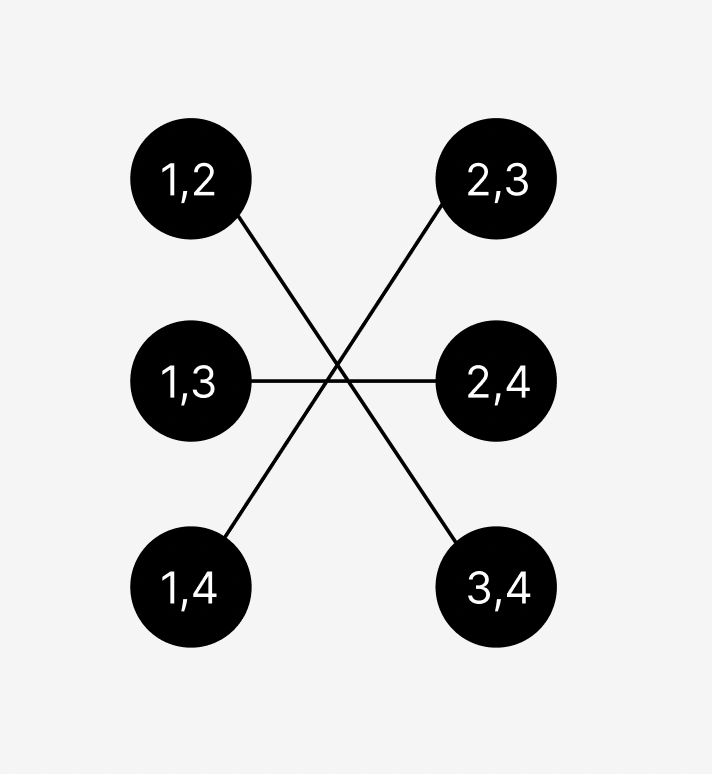
\includegraphics[scale=0.5]{K(4,2).png}}
            \qquad\qquad$K_{4:2}$\label{fig:1}
        \end{minipage}    
        \qquad
        \begin{minipage}{.4\textwidth}
            \centering
            {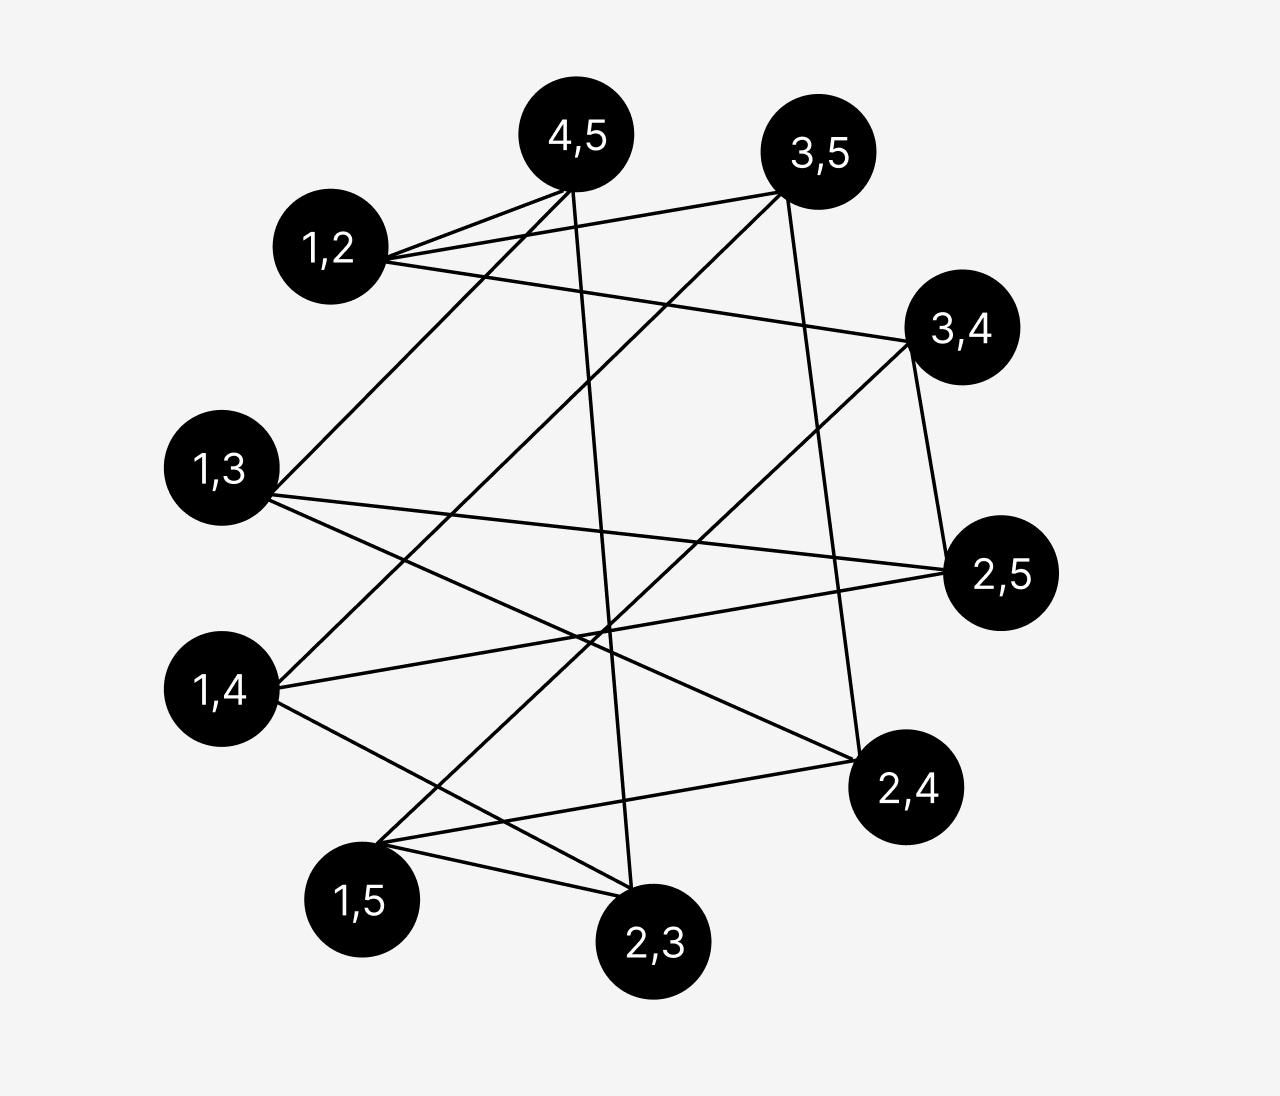
\includegraphics[scale=0.35]{K(5,2).png}}
            \qquad\qquad$K_{5:2}$\label{fig:2}
        \end{minipage}        
    \end{figure} 
    \item By definition, there are a total of ${n\choose r}$ vertices. Then, for any arbitrary $v \in V(K_{n:r})$, there are ${n-r\choose r}$ disjoint vertex (basically just choosing $r$ number of vertices that are not in $v$ already), which would be the neighbors. 
    Hence, for all $v\in V(K_{n:r})$, $d(v) = {n-r\choose r} \Rightarrow \sum\limits_{v\in V}d(v) = {n\choose r}\times {n-r \choose r} \Rightarrow |E(K_{n:r})| = \frac{1}{2}\sum\limits_{v\in V}d(v) = \frac{1}{2}{n\choose r}\times {n-r \choose r}$ [Handshake lemma].
\end{enumerate}
\bigbreak

\textbf{Problem 3.}
\begin{prop}
    Every graph with at least two vertices contains two vertices with the same degree.
\end{prop}
\begin{proof}
    Let $G$ be a graph with $|V(G)|=n$, then for any $v \in V(G)$, $d(v) \leq n-1$. 
    More specifically, $d(v) \in A = \{0 \le m \le n-1: m \in \mathbb{Z}\}$.
    
    However, we have to realize that there cannot exist any pair $v, w \in V(G)$ simultaneously such that $d(v) = 0$ and $d(w) = n-1$ because $\exists w \in V(G)$ such that $d(w) = n-1 \Rightarrow v\in N(w)\Rightarrow d(v)\neq0$, and vice versa.
    
    Hence, in fact $A = \{1 \le m \le n-1: m \in \mathbb{Z}\}$ or $A = \{0 \le m \le n-2: m \in \mathbb{Z}\}$.
    In either case, $|A| = n-1$. Yet, there are $n$ vertices in $V(G)$, so by pigeonhole principle, there must be at least two vertices with the same degree.
\end{proof}
\bigbreak

\textbf{Problem 4.}
\begin{prop}
    Every tournament contains a Hamiltonian path.
\end{prop}
\begin{proof}
    We can easily see that the proposition holds for $n=1,2$ vertices, so they will be omitted here.
    Now, let's prove by induction starting from $n=3$.

    \underline{Base case}: $n=3$.
    \begin{figure}[h]
        \centering
        {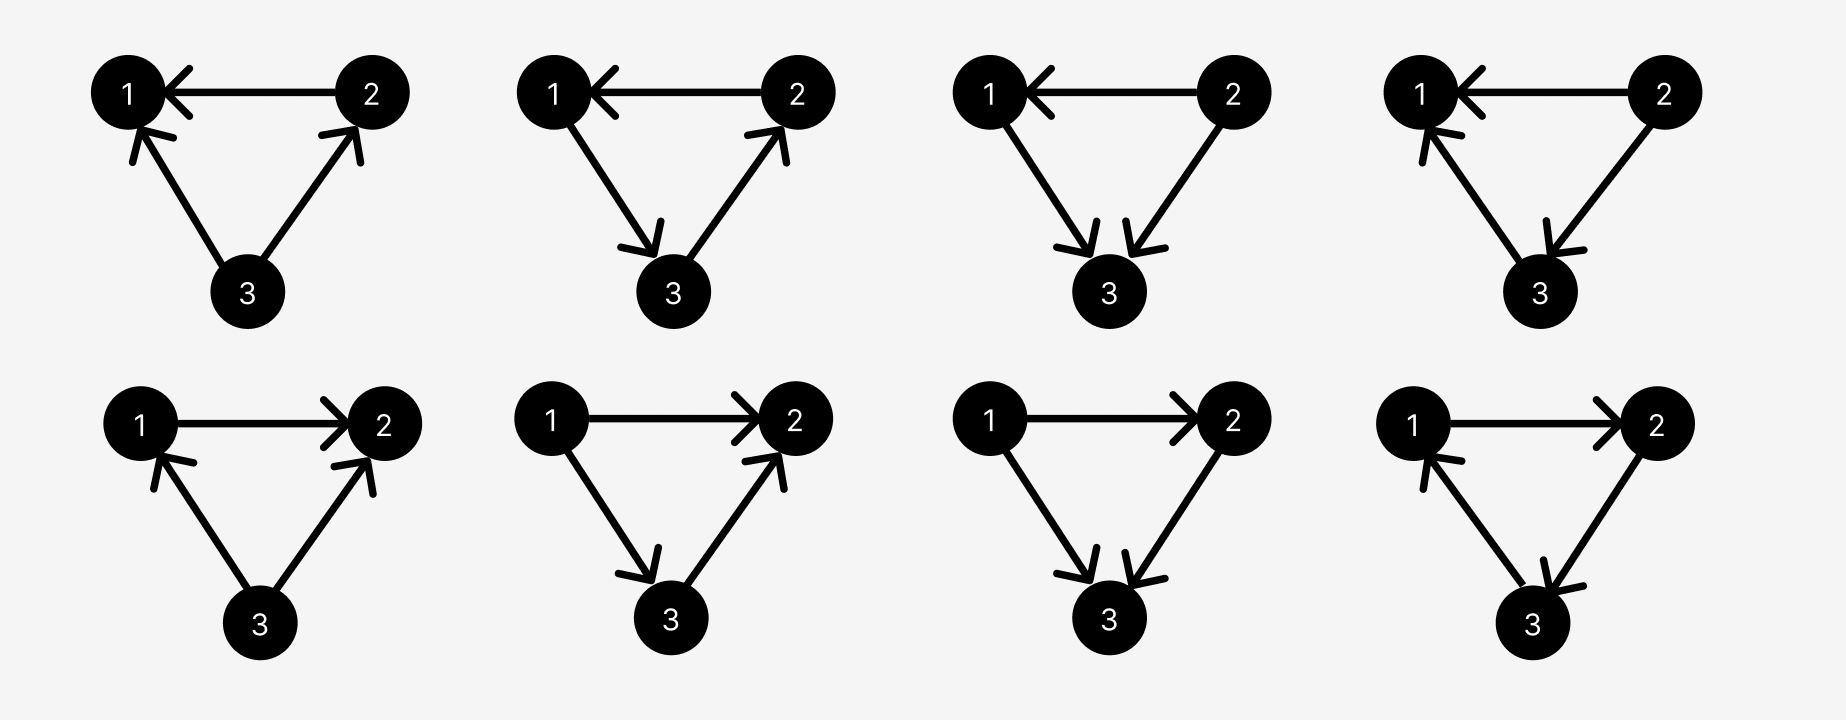
\includegraphics[scale=0.5]{K3_orientations.png}}
        \caption{Orientations of $K_3$}
    \end{figure}

    We can see that every possible orientation of $K_3$ contains a Hamiltonian path.
    Hence, the proposition holds for $n=3$.

    \underline{Inductive step}: assume every tournament with number of vertices $k$ contains a Hamiltonian path.
    
    Let $G$ be a tournament with $|V(G)|=k+1$, we want to prove that $G$ contains a Hamiltonian path.
    First, let's consider the subgraph $G' = G - w$ for which $w$ is an arbitrary vertex in $G$.
    By induction hypothesis, $G'$ contains a directed path containing all of its vertices.
    We can denote the directed path as $P'=(v_1, \cdots, v_i, \cdots, v_k)$.
    Then, there can be three cases for $G$:

    \begin{enumerate}[label=Case \arabic*:]
        \item 
        $(w, v_1)$ is an arc of $G$. 
        Then we know there is a Hamiltonian path in $G$ by adding $w$ to the beginning of $P'$.

        \item
        $(v_k, w)$ is an arc of $G$. 
        Then we also know there is a Hamiltonian path in $G$ by appending $w$ to the end of $P'$.

        \item 
        $(w, v_1)$ and $(v_k, w)$ are both not arcs of $G \Rightarrow$ $(v_1, w)$ and $(w, v_k)$ must be arcs of $G$.
        In other words, $v_1$ is adjacent \emph{to} $w$ and $v_k$ is adjacent \emph{from} $w$.
        Then we know for $1 \le i \le k-1$, there much exist $v_i$ such that $v_i$ is adjacent \emph{to} $w$ and $v_{i+1}$ is adjacent \emph{from} $w$
        because the direction of the arcs between $v_i$ and $w$ must switch for $i \in [1, k]$.
        
        Therefore, we can construct a Hamiltonian path in $G$ by inserting $w$ between $v_i$ and $v_{i+1}$, giving $P$ = $(v_1, \cdots, v_i, w, v_{i+1}, \cdots, v_k)$.
    \end{enumerate}
    
    Hence, we have proved that every tournament with $k+1$ vertices contains a Hamiltonian path.
    
    \underline{By Mathematical Induction}, we have proved that every tournament with $|V| \ge 3$ contains a Hamiltonian path.

    We know that the proposition is indeed also true for $n=1,2$, thus we have proved that every tournament contains a Hamiltonian path.
\end{proof}


\end{document}